    %------------------第五章---------------------------
    \newpage
	\section{超声波接近传感器实物制作与检测}
 \subsection{超声波接近传感器实物制作}
 \subsubsection{超声波接近传感器焊接}
	在完成硬件部分和软件部分的设计之后,就将进行元器件采购、打板、实物焊接制作。如图\ref{PCB实物焊接图}为焊接完成后的实物图。
	\begin{figure}[ht]
	    \centering
	    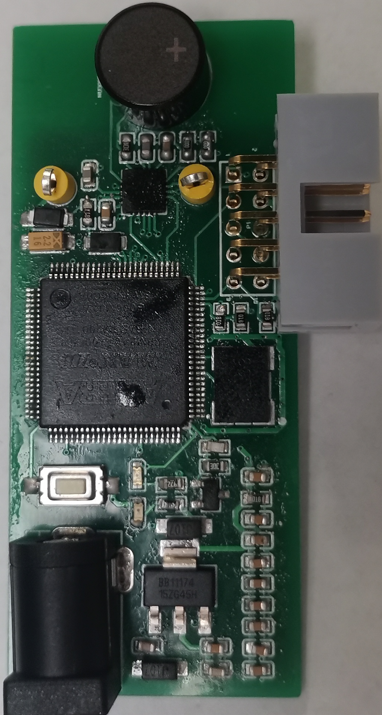
\includegraphics[width=8cm,angle=-90]{figure/physical map.png}
	    \caption{PCB实物焊接图}
	    \label{PCB实物焊接图}
	\end{figure}
 在焊接开始之前,为方便后续的焊接,首先要确定各个元器件的焊接顺序。根据焊接经验,本设计选取的焊接顺序为CPLD芯片->TUSS4470超声驱动芯片->其它贴片器。在确定好焊接顺序后,就可以开始正式焊接。首先清理电路板并检查电路板上是否有问题(例如:短路、断路等),然后用电烙铁焊接好CPLD芯片,并确保各引脚间没有存在虚焊、粘结等情况;焊接完成CPLD芯片后进行驱动芯片的焊接,首先在电路板上涂上焊锡膏,将芯片正确摆放,用热风枪加热焊锡膏使其融化,并轻轻按压芯片使焊盘上锡,最后再用电烙铁将粘结的引脚分离;其它的贴片器件贼按照涂焊锡膏、摆放器件、用热风枪加热的步骤来完成焊接;插件使用电烙铁来焊接。\par
 在完成焊接后,还需检查焊点是否光滑、平整、没有短路和冷焊等问题,使用显微镜或放大镜检查焊点的质量。检查无误后,再用洗板水清洗电路板,去除在焊接过程中多余的松香、锡膏等杂物。清洗完成后,就可以通电进行程序的调试。

\subsubsection{超声波接近传感器调试}
通过示波器对各引脚输出的波形进行检测,然后修改程序,直至每个引脚可以输出正常波形,以下为传感器正常工作时各引脚输出的波形。\par
	\begin{figure}[ht]
	    \centering
	    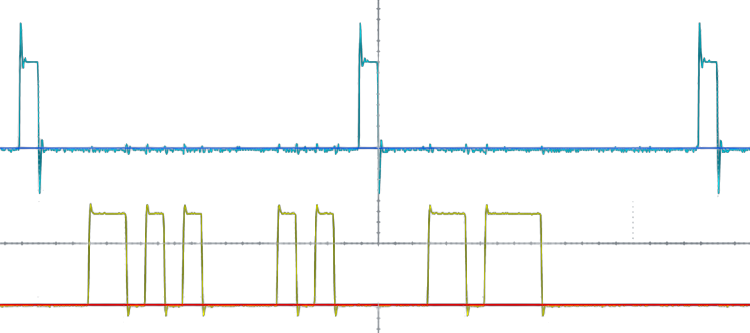
\includegraphics[width=8cm]{figure/debug waveform1.png}
	    \caption{SPI发送数据波形图}
	    \label{SPI发送数据波形图}
	\end{figure}
 如图\ref{SPI发送数据波形图},为采样率100MHz时示波器采集的波形,上方蓝色的为NSS端口的波形,下方黄色的为MOSI端口向驱动芯片发送的配置数据。可以看到,当NSS信号拉低时,MCU开始发送数据,等待一帧数据发送完成后,NSS拉高,并且在下一帧数据发送前,NSS会再次拉低,以实现低-高-低的过程。本设计的程序可以实现连续发送10帧配置数据的功能。
    \begin{figure}[ht]
	    \centering
	    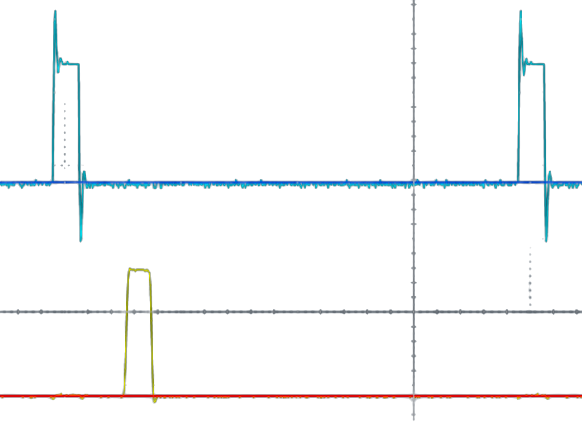
\includegraphics[width=8cm]{figure/debug waveform2.png}
	    \caption{SPI接收数据波形图}
	    \label{SPI接收数据波形图}
	\end{figure}
 图\ref{SPI接收数据波形图}为SPI接收数据的波形图,上方蓝色的波形为NSS端口发送的信号,下方黄色的为MISO端口接收的波形信号。当每次NSS信号拉低时,超声驱动芯片会向MCU返回数据,返回数据的结构如图\ref{SPI数据结构图1}和表\ref{芯片状态表}所示,当传感器正常工作时,只有VDRV\_READY状态位为1,其余位都为0。
   \begin{figure}[ht]
	    \centering
	    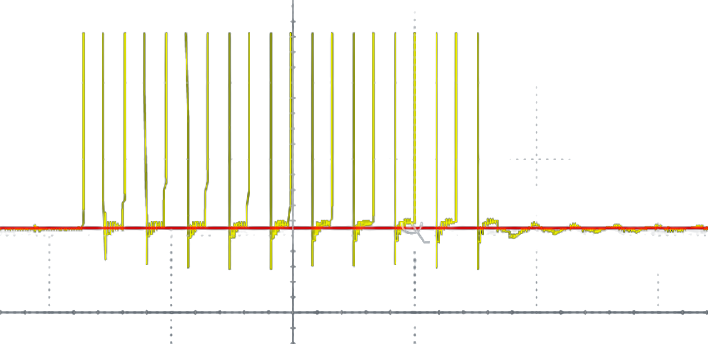
\includegraphics[width=8cm]{figure/debug waveform3.png}
	    \caption{io1、io2引脚波形图}
	    \label{io1、io2引脚波形图}
	\end{figure}
 如图\ref{io1、io2引脚波形图}所示为io1、io2引脚的波形图,两引脚按照IO模式3产生信号,当io1引脚信号拉低时,io2开始产生波形,直到产生指定脉冲数波形后,io1拉高,停止产生波形。
 
 \begin{figure}[ht]
	    \centering
	    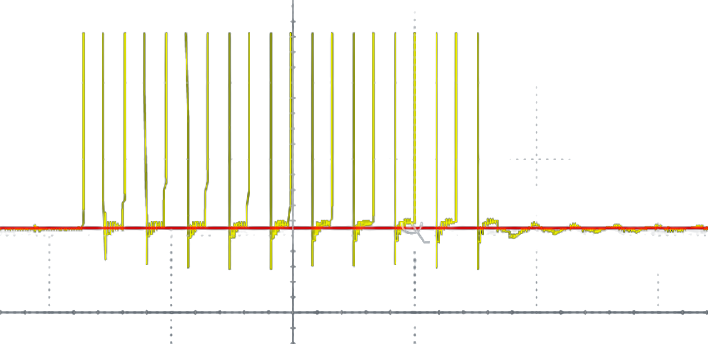
\includegraphics[width=8cm]{figure/debug waveform3.png}
	    \caption{超声探头波形图1}
	    \label{超声探头波形图1}
	\end{figure}
 图\ref{超声探头波形图}为OUTA和OUTB引脚输出的波形,采样频率50MHz,可以看到,探头发出了10个周期频率为300kHz的脉冲波。
  \begin{figure}[ht]
	    \centering
	    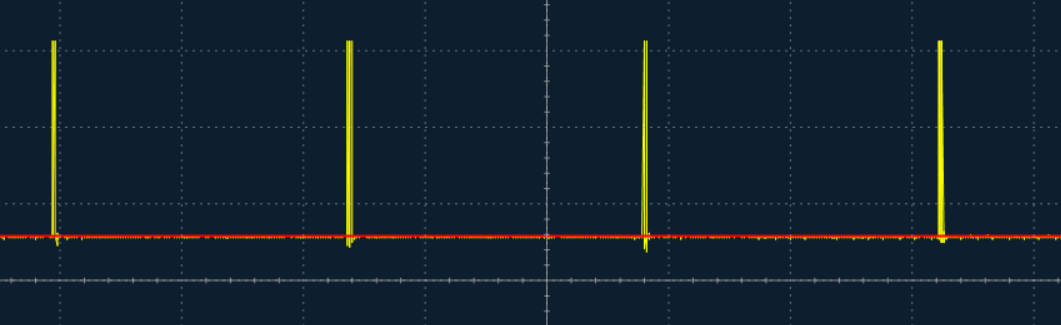
\includegraphics[width=8cm]{figure/debug waveform4.png}
	    \caption{超声探头波形图2}
	    \label{超声探头波形图2}
	\end{figure}
 图\ref{超声探头波形图2}为示波器采样率10MHz时采集到的波形,超声探头连续的发送波形,以10个脉冲为发送周期,每过2.4ms完成一次脉冲的发送。
 \begin{figure}[ht]
	    \centering
	    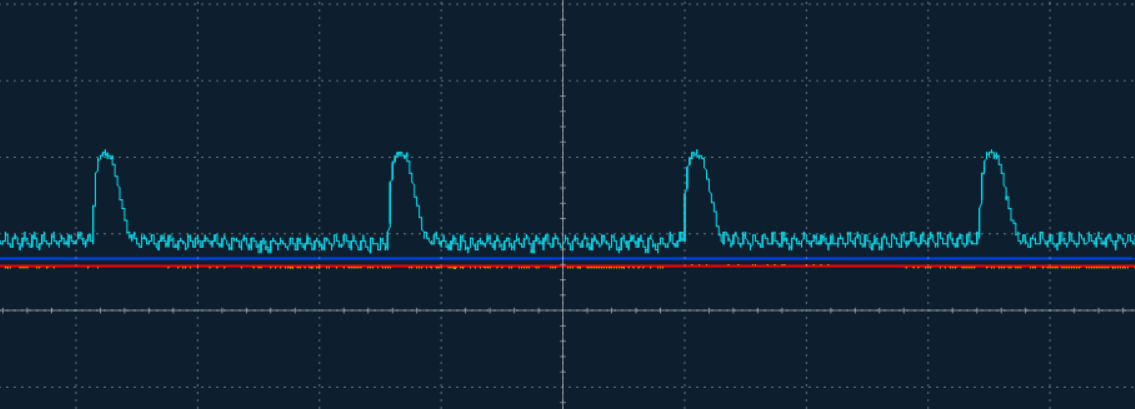
\includegraphics[width=8cm]{figure/debug waveform5.png}
	    \caption{VOUT引脚波形图(无物体遮挡)}
	    \label{VOUT引脚波形图(无物体遮挡)}
	\end{figure}
 图\ref{VOUT引脚波形图(无物体遮挡)}为无物体遮挡的情况下,VOUT引脚输出的波形,采样频率为1MHz。第一个波峰为探头发出脉冲信号时所引起的干扰,在设计检测程序时需要屏蔽该段的信号,经测量,该段信号的持续时间约为发射脉冲后的0.5ms。
 \begin{figure}[ht]
	    \centering
	    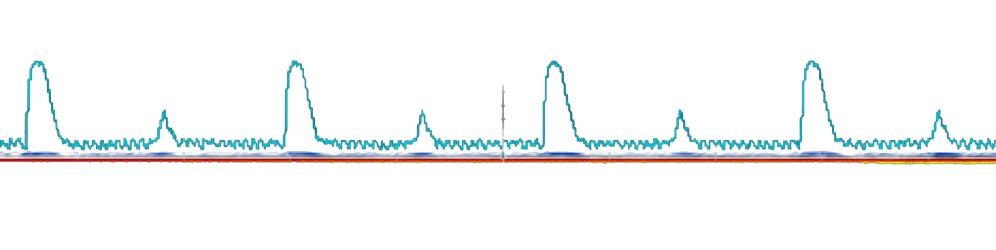
\includegraphics[width=8cm]{figure/debug waveform6.png}
	    \caption{VOUT引脚波形图(有物体遮挡)}
	    \label{VOUT引脚波形图(有物体遮挡)}
	\end{figure}
 图\ref{VOUT引脚波形图(有物体遮挡)}为有物体遮挡时VOUT引脚的输出波形,采样频率为1MHz。当有物体遮挡时,发射的10个脉冲波遇到物体后会进行反射,重新被探头所接收。经过芯片的放大解调处理,形成第二个峰值较低的波峰。
 \begin{figure}[ht]
	    \centering
	    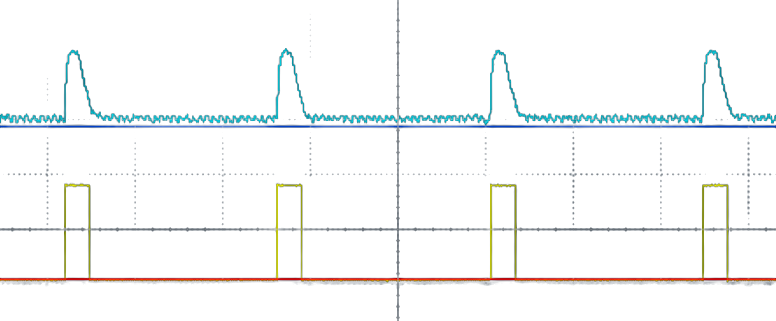
\includegraphics[width=8cm]{figure/debug waveform7.png}
	    \caption{OUT4引脚波形图(无物体遮挡)}
	    \label{OUT4引脚波形图(无物体遮挡)}
	\end{figure}
 图\ref{OUT4引脚波形图(无物体遮挡)}为OUT4引脚的输出波形,采样频率为1MHz。根据芯片手册中所介绍内容,我们不难知道,当VOUT引脚的电压值超过所设定的阈值时,OUT4引脚就会拉高。上图所示波形VOUT的阈值设置为0.9V,当VOUT形成第一个波峰时,电压值超过0.9V的频段OUT4也会拉高。
 \begin{figure}[ht]
	    \centering
	    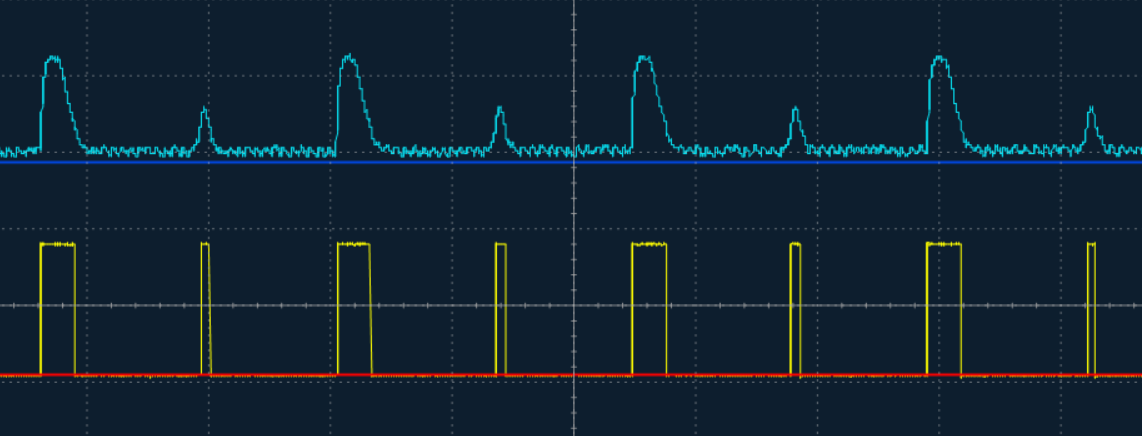
\includegraphics[width=8cm]{figure/debug wave form8.png}
	    \caption{OUT4引脚波形图(有物体遮挡)}
	    \label{OUT4引脚波形图(有物体遮挡)}
	\end{figure}
 图\ref{OUT4引脚波形图(有物体遮挡)}为有物体遮挡时OUT4引脚输出的波形,采样频率为1MHz。当有物体遮挡时,VOUT处理回波产生第二个波峰,而这第二个波峰才是检测所需要用到的有效信号。在这个频段中,VOUT电压值超过所设定的阈值,OUT4第二次拉高,该信号将作为检测物体的重要触发事件。为屏蔽OUT4的第一次拉高信号,在MAIN模块中需要延时一段时间,跳过第一个信号后再开始进行检测,此时只会检测到OUT4的第二个拉高信号,检测有效。

 

\subsection{超声波接近传感器实验}

\subsubsection{实验器材}
在本设计的实验测试当中,采用新型的虚拟示波器,如图所示。该示波器是一种基于计算机的数字示波器,通过采集模拟信号并转换为数字信号,再利用计算机对信号进行处理、显示和分析,实现波形显示的功能。配合功能强大的上位机软件,该示波器具有显示灵活、精度高、波形数据可存储等优点,十分适合本设计的试验调试。\par
其它实验材料如图所示,包括了直尺、12V直流电源供电插头、$100mm\times100mm$的测试板材。

\subsubsection{超声波接近传感器性能参数测试}
在本设计的实验中,对传感器的各性能参数进行了测试,如表所示,有效检测范围为100mm-200mm,传感器精度为1mm,LED检测指示灯刷新的频率为Hz,即每过ms完成一次检测状态的刷新。
 \begin{table}[ht]
        \centering
        \caption{性能参数表}

        \begin{GDUTtable}{\textwidth}{Y Y Y}
            \textbf{参数名 }& \textbf{参数值} &\textbf{单位}    \\ 
            \hline
            检测范围    &   100-200 & mm  \\ 
            检测精度 &  1 & mm  \\\
            检测周期 &  2.4 &ms  \\      
      
            \end{GDUTtable}
        \label{芯片状态表}    
         \end{table}


\subsubsection{超声波接近传感器稳定性测试}
在有干扰的情况下进行性能测试

干扰源选取:可度量的干扰源

在检测周期不变的情况下,调整检测逻辑,观察应对干扰的效果

\subsubsection{不同材料的测试}
将测试物体放置在距离超声波传感器150mm的位置,每次发射脉冲数为8的脉冲,对于不同材料的检测物体进行测试,观察VOUT波形的峰值,测量五次取平均值。实验材料为亚克力板、纸板、陶瓷板、玻璃,实验结果如表所示。
 \begin{table}[ht]
        \centering
        \caption{不同材料测试结果}
        \begin{GDUTtable}{\textwidth}{Y Y Y}
            \textbf{材料类型 }& \textbf{VOUT波形峰值} &\textbf{单位}      \\
            \hline
            亚克力板 & 0.79 &v  \\
            纸板 & 0.78 &v \\
            陶瓷板 & 0.79 &v\\
            玻璃 & 0.8 &v\\
            \end{GDUTtable}
        \label{芯片状态表}    
         \end{table}
根据实验结果,我们可以画出各材料对应回波峰值的折线图,如图所示。通过观察图形,我们可以得知,VOUT回波与物体的材质并无太大关系,当检测物体材质改变时,VOUT引脚输出的波形并没有太大的变化,而与反射脉冲波的强度有关。

\subsubsection{不同脉冲数的测试}
将检测物体放置在距离超声波传感器150mm的位置,改变每次发送脉冲波的脉冲数,观察VOUT波形峰值的变化情况。
亚克力板,脉冲数3,5,7,9,11
纸板
石板
石英玻璃,脉冲数3.5,7,9,11
图中每个数据点都为实验五次取平均值后的结果,可以看到,当每次发射脉冲波的脉冲数越多时,VOUT引脚的峰值就越大。



\subsubsection{不同距离的测试}
以亚克力板作为检测物体,将测试物体放置在距离传感器50mm,100mm,150mm,200mm,250mm的位置,测试其回波信号t值的大小,t值为波峰距离检测周期起点的时间,实验结果如图所示。


当检测距离增加时,VOUT第二个波峰的峰值在不断减小,距离检测起点的时间也在不断增加,与图\ref{VOUT输出}对比,实验结果相近,可以证明传感器脉冲发射检测没有异常。
\subsection{本章小结}
本章介绍了